\documentclass{article}

\usepackage[utf8]{inputenc}
\usepackage{amsmath}
\usepackage{amsfonts}
\usepackage{amssymb}
\usepackage{graphicx}
\usepackage{tikz}
\usetikzlibrary{positioning, shadows}

\title{Computer Systems from a Programmers Perspective}
\author{Thomas Kidane}
\date{\today}

\begin{document}

\maketitle

\section{Chapter 1}


\subsection{Introduction}
This is a collection of my notes from reading Pearson and Hallaron, Computer
System from a Programmers Perspective book. Unfortunately I read the book upto chapter 8 
before starting to write notes, so I will write brief notes on the content upto chapter 8. Covering 
only those I deem important enough to receive a look through again.
We first start off with the simple hello program in C.

\begin{center}
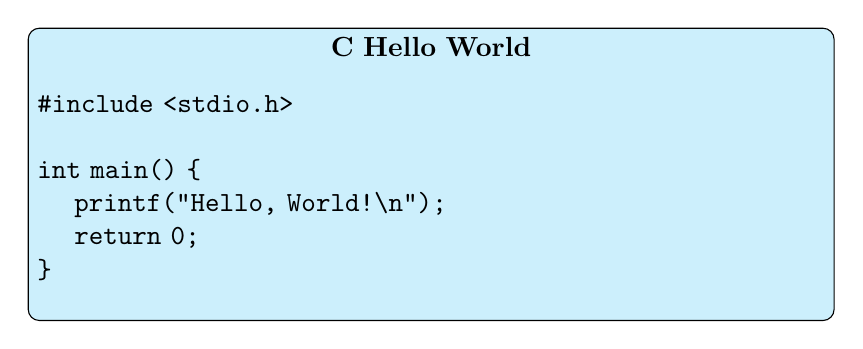
\begin{tikzpicture}
\node[draw, rectangle, rounded corners, fill=cyan!20, text width=10cm, text centered] {
    \textbf{C Hello World}
    \begin{verbatim}
#include <stdio.h>

int main() {
    printf("Hello, World!\n");
    return 0;
}
    \end{verbatim}
};
\end{tikzpicture}
\end{center}

This program is very simple but to actually execute this program requires 
a the interaction of large layer of system components, from the CPU executing 
assembly code, the compiler turning the code in to assemble, the linker linking 
the outputed binary object with the static libraries and putting in runtime memory references
. The whole process if very complicated system is shown in the below diagram.

\begin{center}
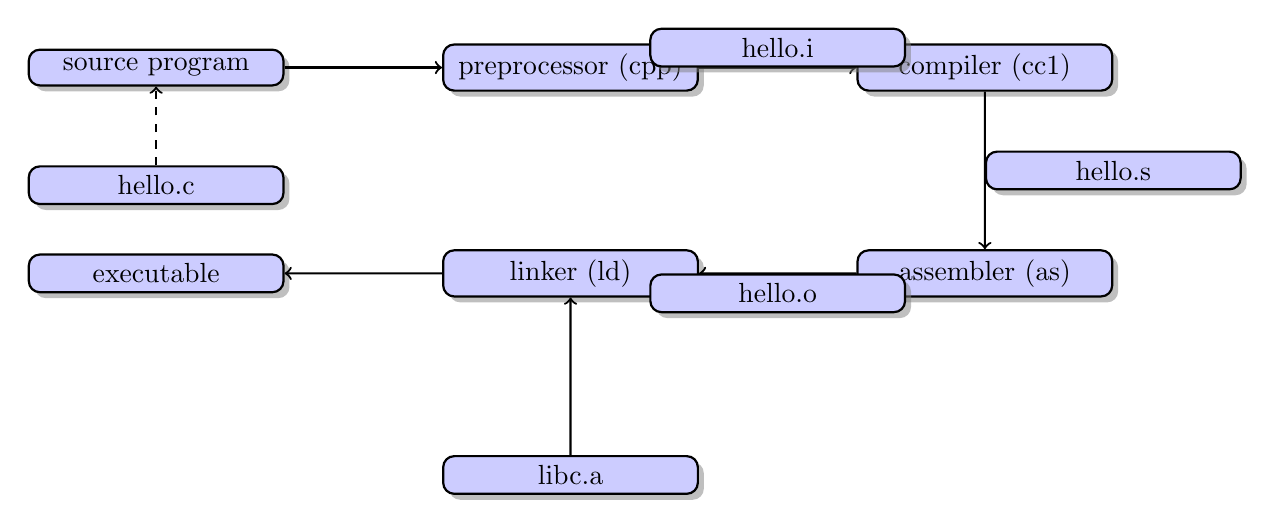
\begin{tikzpicture}[scale=0.7, node distance=2cm, auto, thick, 
    every node/.style={draw, rectangle, rounded corners, fill=blue!20, drop shadow, text centered, text width=3cm}]
    \node (source) {source program};
    \node (preprocessor) [right=of source] {preprocessor (cpp)};
    \node (compiler) [right=of preprocessor] {compiler (cc1)};
    \node (assembler) [below=of compiler] {assembler (as)};
    \node (linker) [left=of assembler, node distance=3cm] {linker (ld)};
    \node (executable) [left=of linker] {executable};

    \draw[->] (source) -- (preprocessor);
    \draw[->] (preprocessor) -- node {hello.i} (compiler);
    \draw[->] (compiler) -- node {hello.s} (assembler);
    \draw[->] (assembler) -- node {hello.o} (linker);
    \draw[->] (linker) -- (executable);

    \node (libc) [below=of linker] {libc.a};
    \draw[->] (libc) -- (linker);

    % Add label pointing to source program
    \node[below=1cm of source, align=center] (source_label) {hello.c};
    \draw[->, dashed] (source_label) -- (source);
\end{tikzpicture}
\end{center}

All of this starts with the gcc command.

\begin{verbatim}
linux> gcc -o hello hello.c
\end{verbatim}

\subsection{Phases of Compilation}

\paragraph{Preprocessing Phase}
\begin{center}
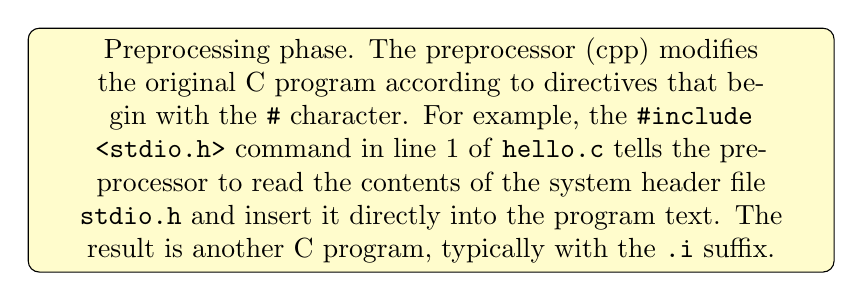
\begin{tikzpicture}
\node[draw, rectangle, rounded corners, fill=yellow!20, text width=10cm, text centered] {
    Preprocessing phase. The preprocessor (cpp) modifies the original C program
    according to directives that begin with the \texttt{\#} character. For example, the
    \texttt{\#include <stdio.h>} command in line 1 of \texttt{hello.c} tells the preprocessor
    to read the contents of the system header file \texttt{stdio.h} and insert it directly
    into the program text. The result is another C program, typically with the \texttt{.i}
    suffix.
};
\end{tikzpicture}
\end{center}

\paragraph{Compilation Phase}
\begin{center}
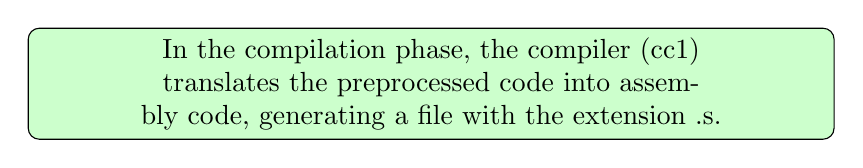
\begin{tikzpicture}
\node[draw, rectangle, rounded corners, fill=green!20, text width=10cm, text centered] {
    In the compilation phase, the compiler (cc1) translates the preprocessed code into assembly code, generating a file with the extension .s.
};
\end{tikzpicture}
\end{center}

\paragraph{Assembly Phase}
\begin{center}
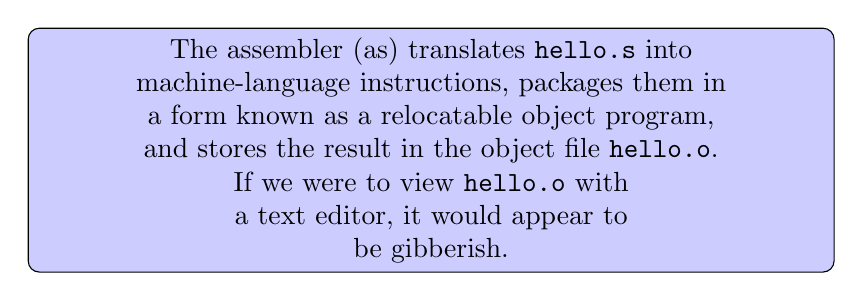
\begin{tikzpicture}
\node[draw, rectangle, rounded corners, fill=blue!20, text width=10cm, text centered] {
    The assembler (as) translates \texttt{hello.s} into machine-language instructions,
     packages them in a form known as a relocatable object program, \\
     and stores the result in the object file \texttt{hello.o}. \\
     If we were to view \texttt{hello.o} with a text editor, it would appear to\\
        be gibberish.  
};
\end{tikzpicture}
\end{center}

\paragraph{Linking Phase}
\begin{center}
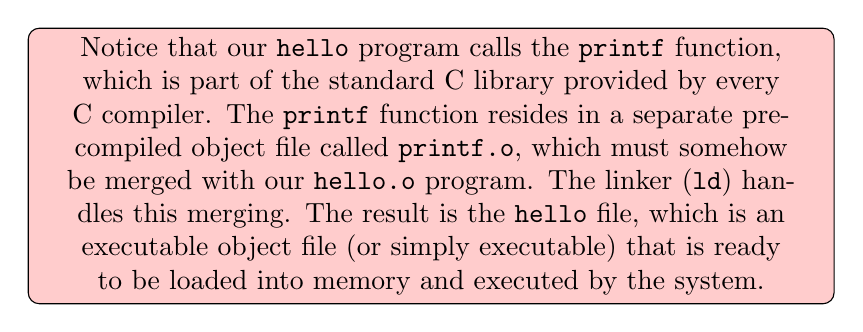
\begin{tikzpicture}
\node[draw, rectangle, rounded corners, fill=red!20, text width=10cm, text centered] {
    Notice that our \texttt{hello} program calls the \texttt{printf} function, which
    is part of the standard C library provided by every C compiler. The \texttt{printf}
    function resides in a separate precompiled object file called \texttt{printf.o}, which
    must somehow be merged with our \texttt{hello.o} program. The linker (\texttt{ld}) handles
    this merging. The result is the \texttt{hello} file, which is an executable object file (or
    simply executable) that is ready to be loaded into memory and executed by
    the system.

};
\end{tikzpicture}
\end{center}

\subsection{Processes}

When a program such as \texttt{hello} runs on a modern system, the operating system
provides the illusion that the program is the only one running on the system. The program such as \texttt{hello} runs on a modern system, the operating system
provides the illusion that the program is the only one running on the system. The
program appears to have exclusive use of both the processor, main memory, and
I/O devices. The processor appears to execute the instructions in the program, one
after the other, without interruption. And the code and data of the program appear
to be the only objects in the system's memory. These illusions are provided by the
notion of a \textit{process}, one of the most important and successful ideas in computer
science.

A \textit{process} is the operating system's abstraction for a running program. Multiple
processes can run concurrently on the same system, and each process appears
to have exclusive use of the hardware. By \textit{concurrently}, we mean that the instructions
of one process are interleaved with the instructions of another process. In
most systems, there are more processes to run than there are CPUs to run them.

This is all allowed by \textit{context switching}. The operating system keeps track of all the state information that the process
needs in order to run. This state, which is known as the \textit{context}, includes information such as the current values of the PC, the register file, and the contents of main
memory. At any point in time, a uniprocessor system can only execute the code
for a single process. When the operating system decides to transfer control from
the current process to some new process, it performs a context switch by saving
the context of the current process, restoring the context of the new process, and 
then passing control to the new process. The new process picks up exactly where
it left off.

\begin{center}
    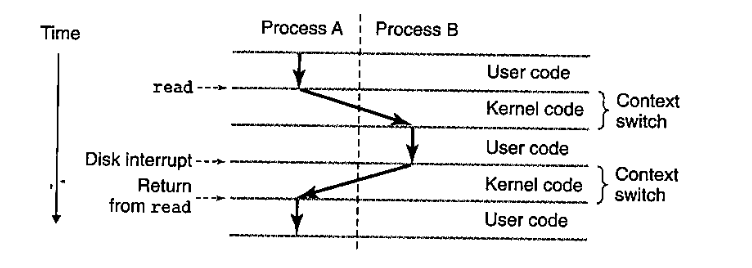
\includegraphics[width=0.8\textwidth]{imgs/pic1.png}  % Adjust width as needed
\end{center}


As the above figure, indicates, the transition from one process to another is managed by the operating system kernel. The kernel is the portion of the operating
system code that is always resident in memory. When an application program
requires some action by the operating system, such as to read or write a file, it
executes a special system call instruction, transferring control to the kernel. The
kernel then performs the requested operation and returns back to the application
program. Note that the kernel is not a separate process. Instead, it is a collection
of code and data structures that the system uses to manage all the \textit{processes}.

\subsection{Threads}

Although we normally think of a process as having a single control flow, in modern
systems a process can actually consist of multiple execution units, called \textit{threads},
each running in the context of the process and sharing the same code and global
data. Threads are an increasingly important programming model because of the
requirement for concurrency in network servers, because it is easier to share data
between multiple threads than between multiple processes, and because threads
are typically more efficient than processes. Multi-threading is also one way to make
programs run faster when multiple processors are available, as we will discuss in

\subsection{Virtual Memory}

\begin{center}
    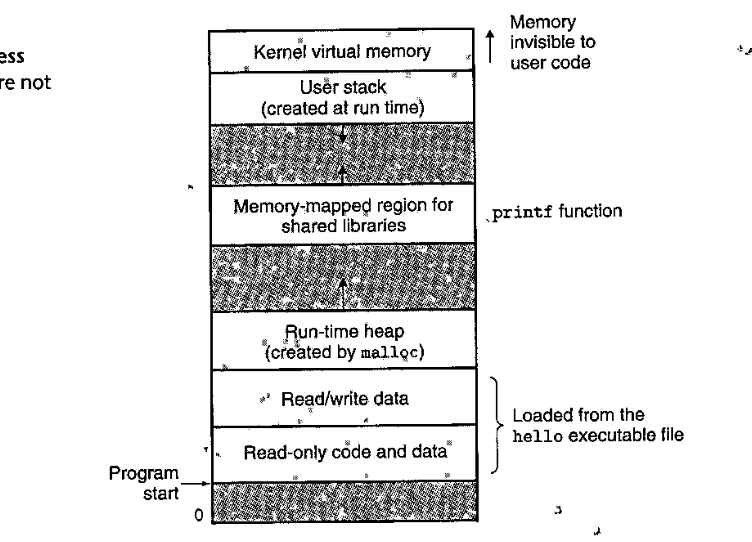
\includegraphics[width=0.8\textwidth]{imgs/pic2.png}  % Adjust width as needed
\end{center}

Virtual memory is an abstraction that provides each process with the illusion that it
has exclusive use of the main memory. Each process has the same uniform view of
memory, which is known as its virtual address space. The virtual address space for
Linux processes is shown in the above figure(Not drawn to scale). (Other Unix systems use a similar layout.)
In Linux, the topmost region of the address space is reserved for code and data
in the operating system that is common to all processes.
The lower region of the
address space holds the code and data defined by the user's process. Note that
addresses in the figure increase from the bottom to the top.

The virtual address space seen by each process consists of a number of well-
defined areas, each with a specific purpose. You will learn more about these areas
later in the book, but it will be helpful to look briefly at each, starting with the
lowest addresses and working our way up:

\textit{Program code and data. Code begins at the same fixed address for all processes,}
followed by data locations that correspond to global C variables. The code. and
data areas are initialized directly from the contents of an executable object
file-in our case, \texttt{hello} executable.\\

\textit{Heap} The code and data areas are followed immediately by the-run-time \textit{heap}.
Unlike the code and data areas, which are fixed in size once the process begins 
running, the heap expands and contracts dynamically at run time as a result
of calls to C standard library routines such as malloc and free.\\

\textit{Shared libraries} Near the middle of the address space is an area that holds the
code and data for shared libraries such as the C standard library and the math
library. The notion of a shared library is a powerful but somewhat difficult
concept.\\

\textit{Stack} At the top of the user's virtual address space is the user stack that
the compiler uses to implement function calls. Like the heap, the user stack
expands and contracts dynamically during the execution of the program. In
particular, each time we call a function, the stack grows. Each time we return
from a function it contracts.

\textit{Kernel virtual memory} The top region of the address space is reserved for the
kernel. Application programs are not allowed to read or write the contents of
this area or to directly call functions defined in the kernel code. Instead, they
must invoke the kernel to perform these operations.\\


For virtual memory to work, a sophisticated interaction is reqµired between
the hardware and the operating system software, including a hardware translation
of every address generated by the processor. The basic idea is to store the contents
of a process's virtual memory on disk and then use the main memory as a cache
for the disk. 


\subsection{Files}

A \textit{file} is a sequence of bytes, nothing more and nothing less. Every I/O device,
including disks, keyboards, displays, and even networks, is modeled as a file. All
input and output in the system is performed by reading and writing files, using a
small set of system calls known as Unix I/O.\\

This simple and elegant notion of a file is nonetheless very powerful because
it provides applications with a uniform view of all the varied I/O devices that
might be contained in the system. For example, application programmers who
manipulate the contents of a disk file are blissfully unaware of the specific disk
technology. Further, the same program will run on different systems that use
different disk technologies.

\subsection{Systems Communicate with Other Systems
Using Networks}

\begin{center}
    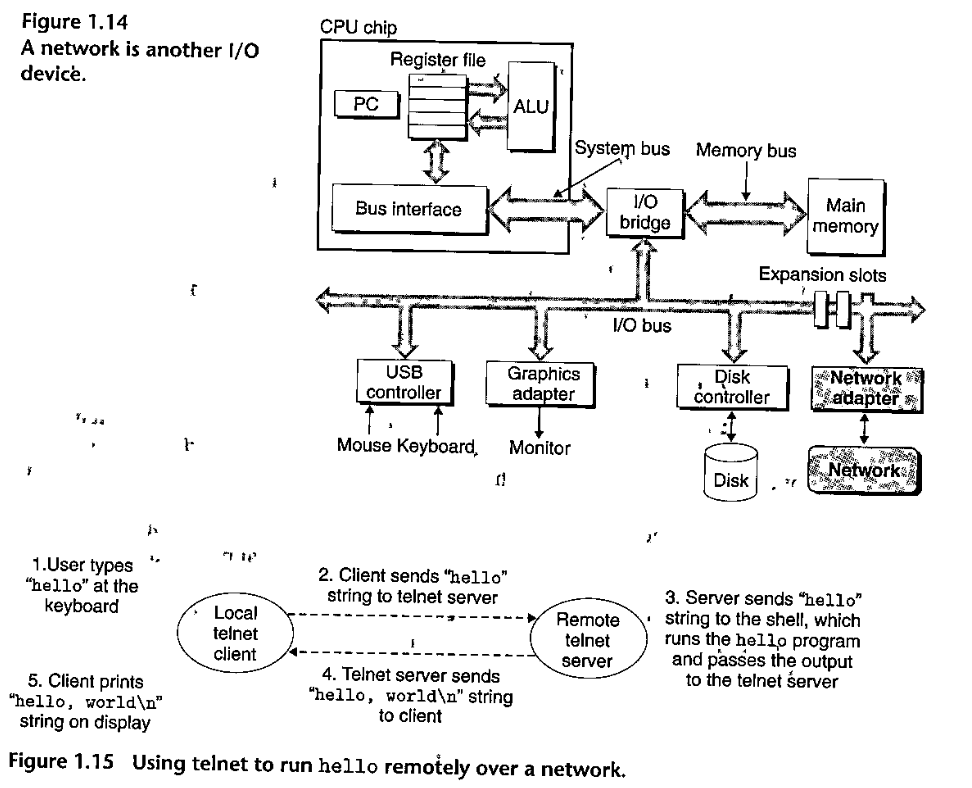
\includegraphics[width=0.8\textwidth]{imgs/pic3.png}  % Adjust width as needed
\end{center}

Up to this point in our tour of systems, we have treated a system as an isolated
collection of hardware and software. In practice, modern systems are often linked
to other systems by networks. From the point of view of an individual system, the
network can be viewed as just another I/O device, as shown in Figure 1.14. When
the system copies a sequence of bytes from main memory to the network adapter,
the data flow across the network to another machine, instead of, say, to a local
disk drive. Similarly, the system can read data sent from other machines and copy
these data to its main memory.\\

With the advent of global networks such as the Internet, copying information
from one machine to another has become one of the most important uses of
computer systems. For example, applications such as email, instant messaging, the
World Wide Web, FTP, and telnet are all based on the ability to copy information
over a network.

\subsection{Important Themes}

\subsubsection{Amdahl's Law}

This law describes the amount of performance that can be gained from improving 
one part of a system. 

The main idea is that when we speed up one part of a system, the effect on the overall system performance depends on both how significant this part was and how much it sped up. Consider a system in which executing some application requires time \( T_{\text{old}} \). Suppose some part of the system requires a fraction \( \alpha \) of this time, and that we improve its performance by a factor of \( k \). That is, the component originally required time \( \alpha T_{\text{old}} \), and it now requires time \( \frac{\alpha T_{\text{old}}}{k} \). The overall execution time would thus be
\[
T_{\text{new}} = (1 - \alpha) T_{\text{old}} + \frac{\alpha T_{\text{old}}}{k} = T_{\text{old}} \left[ (1 - \alpha) + \frac{\alpha}{k} \right]
\]
From this, we can compute the speedup \( S = \frac{T_{\text{old}}}{T_{\text{new}}} \) as
\[
S = \frac{1}{(1 - \alpha) + \frac{\alpha}{k}}
\]
As an example, consider the case where a part of the system that initially consumed 60\% of the time (\( \alpha = 0.6 \)) is sped up by a factor of 3 (\( k = 3 \)). Then we get a speedup of
\[
S = \frac{1}{0.4 + \frac{0.6}{3}} \approx 1.67
\]
Even though we made a substantial improvement to a major part of the system, our net speedup was significantly less than the speedup for the one part. This is the major insight of Amdahl's Law: to significantly speed up the entire system, we must improve the speed of a very large fraction of the overall system.

\subsection{Concurrency and Parallelism}

We use the term concurrency to refer to the general concept of a system with
multiple, simultaneous activities, and the term parallelism to refer to the use of
concurrency to make a system run faster. Parallelism can be exploited at multiple
levels of abstraction in a computer system. We highlight three levels here, working
from the highest to the lowest level in the system hierarchy.

\subsubsection{Thread-level Concurrency}
Building on the process abstraction, we are able to devise systems where multiple
programs execute at the same time, leading to concurrency. With threads, we
can even have multiple control flows executing within a single process. Traditionally, this concurrent execution was
only simulated, by having a single computer rapidly switch among its executing
processes, much as a juggler keeps multiple balls flying through the air. This form
of concurrency allows multiple users to interact with a system at the same time,
such as when many people want to get pages from a single Web server. It also
allows a single user to engage in multiple tasks concurrently, such as having a
Web browser in one window, a word processor in another and streaming music
playing at the same time. Until recently, most actual computing was done by a
single processor, even if that processor had to switch among multiple tasks. This
configuration is known as a uniprocessor system.\\
When we construct a system consisting of mulitple processors all under the
control of a single operating system kernel, we have a multiprocessor system.
Such systems have been available for large-scale computing since the 1980s, but
they have more recently become commonplace with the advent of multi-core
processors aiid hyperthreading. Figure 1.16 shows a taxonomy of these different
processor types.\\
Multi-core processors have several CPUs (referred to as ``cores'') integrated
onto a single integrated-circuit chip. Figure 1.17 illustrates the organization of a

\begin{center}
    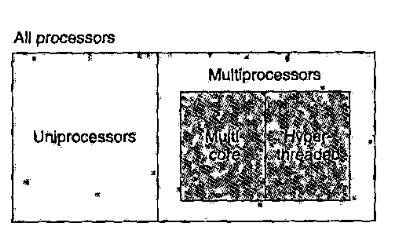
\includegraphics[width=0.8\textwidth]{imgs/pic4.png}  % Adjust width as needed
\end{center}

\begin{center}
    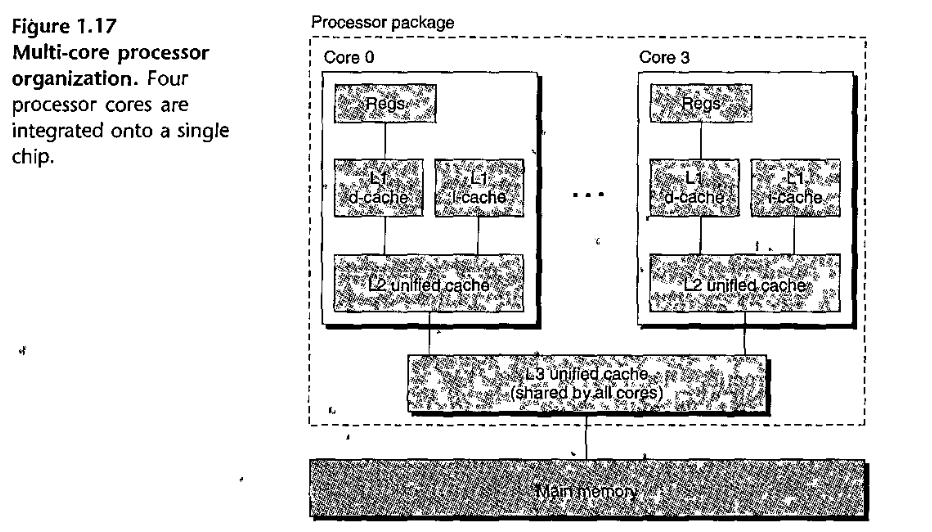
\includegraphics[width=0.8\textwidth]{imgs/pic5.png}  % Adjust width as needed
\end{center}

typical multi-core processor, where the chip has four CPU cores, each with its
own L1 and L2 caches, and with each L1 cache split into two parts - one  to hold
recently fetched instructions and one fo hold data. The cores share higher levels of
cache as well as the interface to main memory. typical multi-core processor, where the chip has1four CPU cores, each with its
own L1 and L2 caches, and with each L1 cache split into two parts-<me to hold
recently fetched instructions and one fo hold data. The cores share higher levels of
cache as well as the interface to main memory.

Hyperthreading, sometimes called simultaneous multi-threading, is a tech-
nique that allows a single CPU to execute multiple flows of control. It involves
having multiple copies of some of the CPU hardware, such as program counters
and register:files, while having only single copies of other parts of the hardware,
such as the units that perform floating-point arithmetic. Whereas a conentional
processor requires around 20,000 clock cycles to shift between different threads,
a hyperthreaded processor decides which of its threads to execute on a cycle-by-
cycle basis. It enables the CPU to take better advantage of its processing resources.
For example, if one thread must wait for some data to be loaded into a cache, the
CPU can proceed with the execution of a different thread. As an example, the Intel 
Core i7 processor can have each core executing two threads, and so a four-core
system cah actually execute eight threads in parallel.\\

The use of multiprocessing can improve system performance in two ways.
First, it reduces the need to simulate concurrency when performing multiple tasks.
As mentioned, even a personal computer being used by a single person is expected
to perform many activities concurrently. Second, it can run a single application
program faster, but only if that program is expressed in terms of multiple threads
that can effectively execute in parallel. Thus, although the principles of concurrency
have been formulated and studied for over 50 years, the advent of multi-core
and hyperthreaded systems has greatly increased the desire to find ways to write
application programs that can exploit the thread-level parallelism available with 
the available hardware.


\subsubsection{Instruciton Parallelism}
At a much lower level of abstraction, modern processors can execute multiple
instructions at one time, a property known as instruction-level parallelism. For
example, early microprocessors, such as the 1978-vintage Intel 8086, required
multiple (typically 3-10) clock cycles to execute a single instruction. More recent
processors can sustain execution rates of 2-4 instructions per clock cycle. Any
given instruction requires much longer from start to finish, perhaps 20 cycles or
more, but the processor uses a number of clever tricks to process as many as 100
instructions at a time. The stages can operate in parallel, working on different parts of
different instructions. We will see that a fairly simple hardware design can sustain
an execution rate close to 1 instruction per clock cycle.
Processors that can sustain execution rates faster than 1 instruction per cycle
are known as superscalar processors. Most modern processors support superscalar
operation.

\subsubsection{Single Instruction, Multiple-Data (SIMD) Parallelism}
At the lowest level, many modern processors have Special hardware that allows
a single instruction to cause multiple operations to be performed in parallel, a
mode known as single-instruction, multip.fe-data (SIMD) parallelism. Fpr example,
recent generations of Intel and AMD,processors have instructions that can add 8
pairs of single-precisjon floating-pint-numbers (C data type float) in parallel.
These SIMD instructions are provided mostly to speed up applications that
process image, sound, and video data. Although some compilers attempt to automatically
extract SIMD parallelism from C progams, a more reliable method is to
write programs using special vector data types supported in compilers such as GCC.

\subsection{Summary}

A computer system consists of hardware and systems software that cooperate
to run application programs. Information inside the computer is represented as
groups of bits that are interpreted in different ways, depending on the context.
Programs are translated by other programs into different forms, beginning as
ASCII text and then translated by compilers and linkers into binary executable
files.
Processors read and interpret binary instructions that are stored in main memory.
Since computers spend most of their time copying data between memory, I/O
devices, and the CPU registers, the storage devices in a system are arranged in a hi-
erarchy, with the CPU registers at the top, followed by multiple levels of hardware
cache memories, DRAM main memory, and disk storage. Storage devices that are
higher in the hierarchy are faster and more costly per bit than those lower in the 
hierarchy. Storage devices that are higher in the hierarchy serve as caches for
devices that are lower in the hierarchy. Programmers can optimize the performance
of their C programs by understanding and exploiting the memory hierarchy.\\

The operating system kernel serves as an intermediary between the applica-
tion and the hardware. It provides three fundamental abstractions: (1) Files are
abstractions for I/O devices. (2) Virtual memory is an abstraction for both main
memory and disks. (3) Processes are abstractions for the processor, main meniory,
and I/O devices.\\

Finally, networks provide ways for computer systems to communicate with
one another. From the viewpoint of a particular system, the network is just another
I/O device.

\section{Information Representation}

\subsection{Little Endian vs Big Endian}

Most Computers are currently byte addressed, so an address of the computer points to a byte of information.
Most addressing works this way because it is architecturally very hard for the computer to address single bits, 
even the boolean in c is actually just a char(8 bits, this is actually implementation dependent but at the time of writing, 
this is the case). So the addresses are aligned byte by byte, which leads to big vs little endian.

A big endian system means that the computer puts the most significant number at the front, and the less significant
digits to the right(or higher order bits are at smaller addresses, which less significant bits are at larger address values). This method is how I intuitevly write it.
On the other hand in a little endian machine, the lower order \textbf{bytes} come first(not bits). In the memory they are ordered based on bytes, so while 
the lower order bytes come first, inside those bytes the bits are actually in the normal order, so the endianness only affects the order of bytes.

Most computers out there are currently little endian.

\subsection{Integer and Floating point representation}

The normal unsigned integer is represented just as how you would think, while the signed integers usually use a 2-complement numbering system.
In this numbering system the first bit is actually negative. So if the number is 4 bits, like 1010, then it the first bit actually determines whether you 
add $-8$, to the final number in base 10 representation. In this case the number would $ -6 = (-8)*(1)+(4)*(0)+(2)*(1)+(1)*(0)$. This system allows you to index 
from $(-2^{b}) - (2^{b}-1)$, the decrement in the positive direction is because all 0 means 0. An interesting fact that causes this representation to be universal is, if you add 
a number to it negative using just a normal base addition, then the result you will get will be $0$ because the last bit overflows. The way to turn an integer into its negative is 
to first invert all its bits and just add 1.

\subsection{Shifting}

The $>>$ or $<<$ operator in c and c++ can be used to shift the bits in a number of any piece of bits. There are 2 types of right shift $>>$. Either logical shift or arthimetic shifts.
The arthimetic shifts preserve sign by replicating the last bit, while logical shift just add zeros at the end, which one you have is implementation and language dependent(Java and Python) 
both support bit shifting.

\subsection{Floating Point Numbers}

The IEEE standard on floating points numbers allows us to represent normalized values in this format.
\begin{align*}
  signbit(1bit) \; exp(exponent, is an unsigend that is shifted down ward by 127 \\for 32 bit(float is usually 32 bits) and 1023 for 64 bit doubles). \;\\ frac (22 bits for 32 bit and 52 bits for 64 bit).\\
  s \; exp \; frac
\end{align*}

In this representation there is an implied 1 before the frac, while in denormalized number(when the exp becomes all 0) there is no implict 1, and the numbers become very close to 0.

There are also special values, when the exponent value becomes all 1, and the frac is all 0, the number is either $-\infty$ or $\infty$ depending on the sign. An $s=0$ corresponds to a 
positive number. There you have exp that is all 1, and frac that is not all 0, you get a $NaN$(Not a number). The infinites could result from overlfow, but the $NaN$ can result from 
an operation that is not defined.

\section{Machine Level Representation}

The $IA32$ is the predecessor of x86-64. Systems that use x86-64 usually support $IA32$ in backward compatibility mode and there systems that exclusively only support $IA32$.
So there are still a lot of software is made for IA32. 

The CPU can only understand bits, so the we compile out programs to a level that the computer can understand, we do this by using assembly language and the CPU ISA.
The ISA(Instruction Set Architecture) tells you what the CPU can do, not how it does it sorta like an API. When a C code turns to assembly code it runs through a couple stages of processsing.

You can use a dissambler to see the byte level of a CPU. Trying to read Assembly is trying to reverse engineer. Due to its origin as a 16 bit architecture that later expanded to 32 bit  one. Intel uses the term "word" to refer to a 16bit data type. The CPU has registers and you primarily work wtih the registers to operate. You also have 
access to instructions that allow you to transfer data between the register and the memory(Which uses caches and virtaul memory, we will get to that later).

When the CPU executes a program it has a stack and a heap. The stack is just that, a stack where  you can put stop on it and pop it off. Confusingly the stack starts at a very high memory address(that is random each time) and grows downward, so you decrement the stack pointer to increase the stack, this also how subroutines and functions are called. The heap is just any memory that you ask the OS to allocate to you, and it usually grows upward. If you do infinite recursion that stack will eventually run out and hit something below, that is when you get 
stack overflow.

There also certain nuances with load and store operations, but you can lookup that detail in the specific ISA you reading. There also control instructions that change the flow of 
the program, this instructions change the position of the program counter(which determines what instruction will be exectued next). There are also stages to instruction execution(The fetch phase, decoding stage, execution stage, memory stage, write back stage). Fetch, and decode are self explantory while execution stage means any instruction that uses the ALu, while the memory means writing to memory and writeback is for registers. Usually you can pipeline the processor to execute multiple different stages of the different instructions at the same time.


There are also condition codes, which determine whether the condition is satisfied when doing a branch instruction. There is also the jump instruction that jumps to a specific address. Through this operations you can implement stuff like if and fors. There things called Data Transfers that allow the CPU to execute both sides of an if at the same time and just change the data if the condition is satisfied or not, the CPU will do this if it can, and where the program doesn't have any side effects.

All the data structures in a program language are just bits to the CPU, arrays are just continous sections of memory. Multidimentional arrays are also just a long sequence of memory and 
you access them by doing indexing math when you do the indexing, you can do this by using pointer arthimetic. The array access notation [] just does the pointer mathematics for you.

There are also structures which allow you to put multiple data types in one object, this are represented in the memory as just a continous memory and you can access the individual properties by just indexing.

If you are going to work with c, use gdb to understand where you fucked up.

There also stack overflow attacks that exploit the position of the stack to access unauthorised information and unwanted instructions. You can defend against this by randomizing the position of the stack.

The buffer overflow attacks are done by making the program do an instruction it didn't intend to do by injecting exploit code that affects the stack. You can also check if the stack is corrupted to fight against bufferoverflow attacks.

When the CPU exectutes code from different data types it usually increases the precision of the less precise data type, so from int to long long and from float to double. 
\end{document}
